\documentclass[aspectratio=169]{beamer}
\usepackage{graphicx}

\usetheme{default}

\graphicspath{{ .} }

\title{CORE-Storage}
\subtitle{Concepts and uses}
\author{
	Marius Dieckmann\inst{1,2,3}\newline\url{Marius.Dieckmann@computational.bio.uni-giessen.de}
}

\institute[shortinst]{\textsuperscript{1} Justus-Liebig-Universität Gießen \and \inst{2} NFDI4Biodiversity \and \inst{3} de.NBI}

\begin{document}
	\begin{frame}[plain]
		\maketitle
	\end{frame}
	\begin{frame}
		\begin{figure}
			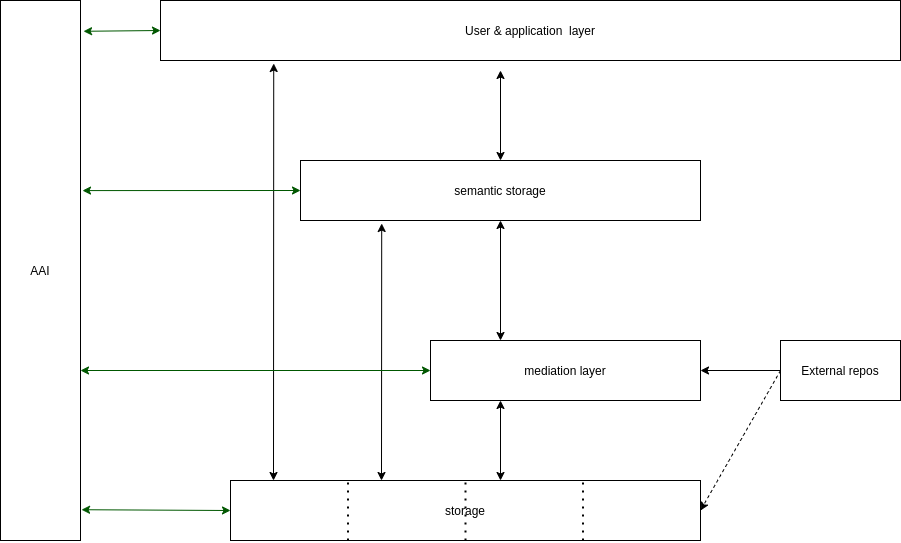
\includegraphics[scale=0.52]{../../images/RDCConcept.png}
		\end{figure}
	\end{frame}

	\begin{frame}{Basic concept}
		\begin{itemize}
			\item API based scalable data management system
			\item Simple data structure consistent versioning
			\item Versioning schema based on semantic versioning
			\item Object history (no implemented)
			\item gRPC API with pre-generated clients stubs
			\item HTTP-REST gateway with OpenAPI documentation
			\item Update event notification via event streaming
			\item Search engine for JSON based metadata
		\end{itemize}
		
	\end{frame}
	\begin{frame}{NFDI4Biodiversity Multicloud}
		\begin{figure}
			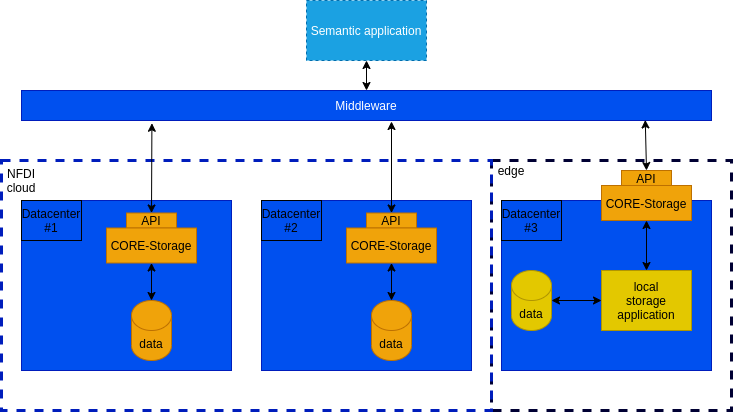
\includegraphics[scale=0.52]{../../images/NFDIMulticloudconcept.png}
		\end{figure}
	\end{frame}
	\begin{frame}{NFDI4Biodiversity Dataflow}
		\begin{figure}
			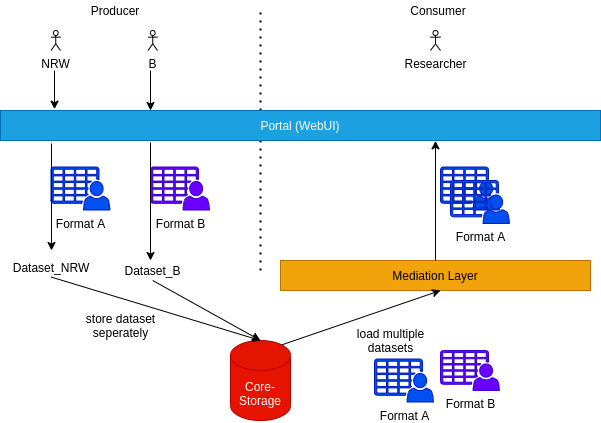
\includegraphics[scale=0.52]{../../images/DataFlowOdonata.png}
		\end{figure}
	\end{frame}
\end{document}